% This LaTeX was auto-generated from MATLAB code.
% To make changes, update the MATLAB code and export to LaTeX again.

\documentclass{article}

\usepackage[utf8]{inputenc}
\usepackage[T1]{fontenc}
\usepackage{lmodern}
\usepackage{graphicx}
\usepackage{color}
\usepackage{hyperref}
\usepackage{amsmath}
\usepackage{amsfonts}
\usepackage{epstopdf}
\usepackage[table]{xcolor}
\usepackage{matlab}
\usepackage[paperheight=795pt,paperwidth=614pt,top=72pt,bottom=72pt,right=72pt,left=72pt,heightrounded]{geometry}

\sloppy
\epstopdfsetup{outdir=./}
\graphicspath{ {./Tracking_live_media/} }

\begin{document}

\matlabtitle{Signal after MAX2771}

\begin{matlabcode}
%rawdata = randi([0 1], [1 50e3]); 
%rawdata = [1 0 1 1 0 0 1 0 0 1 1 0 0 1 1];
rawdata = repmat([1 0 1 0 0 1 1 0 1 0],1,35);

fca     = 1.023e6;          % C/A code frequency
%fc      = 1575.42e6;        % Carrier frequency
fs      = 20*fca;
sv_id   = 1;                % Satellite Vehicle ID
n       = 1;                % BPSK(1) fc = n*1.023e6; %code rate BPSK(n) 
%                               spreading code rate n*1.023 MHz
codeLength = round(1023/n); 

fdoppler = [100, 300, -200, -500];
ca_codes = [ 1,  8,  20, 12];
code_phase = [200, 30, 834, 514];

 Rsignal = 2*( ...
             .25*Received_Simplified(rawdata,fca,fs,fdoppler(1) ...
             ,ca_codes(1),1,code_phase(1)) + ...
           ...
           .25*Received_Simplified(rawdata,fca,fs,fdoppler(2), ...
           ca_codes(2),1,code_phase(2)) + ...
           ...
           .25*Received_Simplified(rawdata,fca,fs,fdoppler(3), ...
           ca_codes(3),1,code_phase(3)) + ...
           ...
           .25*Received_Simplified(rawdata,fca,fs,fdoppler(4), ...
           ca_codes(4),1,code_phase(4)));

%Rsignal = 4*(.25*Received_Simplified(rawdata,fca,fs, ...
%               fdoppler(1),ca_codes(1),1,0) + ...
%            .25*Received_Simplified(rawdata,fca,fs, ...
%               fdoppler(4),ca_codes(4),1,514));

%Rsignal = 2*(Received_Simplified(rawdata,fca,fs, ...
%              fdoppler(1),ca_codes(1),1,code_phase(1)));

[I,Q, clk] = MAX2771_simplified(Rsignal, fs, round(2), true);

clear Rsignal;
\end{matlabcode}


\matlabheading{Defining the PLL tracking loop}


\begin{matlabcode}
IQ = I + 1i*Q;

gc_full = data_mapper(gold_code_L1(codeLength,1));
gc_full = expand(gc_full,20*length(rawdata));
gc_full = upsampler(gc_full,length(IQ)/length(gc_full));
gc_length = length(gc_full);

cd_phase = round(code_phase(1)*10*.985);
spacing = length(IQ)/(2*20*length(rawdata)*1023);
block_size = length(IQ)/(20*length(rawdata));

[IE, QE, IP, QP, IL, QL] = deal(zeros(1,length(IQ)/block_size));

omega = 0.9*fdoppler(1);

T_PID = block_size/clk;
filt_I_PLL = 0;
Ki_PLL = .005;
Kp_PLL = .2;
Kd_PLL = 1e-4;

IQ_data = zeros(1,length(IQ));
nco_out = zeros(1,length(IQ));
pd_out = zeros(1,length(IQ)/block_size);
phase_ramp = 0;

% Filtro do DLL a ser ajustado
filt_I_DLL = 0;
Ki_DLL = 2;
Kp_DLL = 4;
Kd_DLL = 1;
cd_out = zeros(1,length(IQ)/block_size);
DLL_filter = zeros(1,length(IQ)/block_size);
ca_phase_rec = [cd_phase zeros(1,length(IQ)/block_size)];

for i = 1:length(IQ)/block_size
    idx = (1:block_size) + (i - 1) * block_size;
    phase_ramp = 2.*pi.*omega(i).*(idx-1)./clk;
    nco_out(idx) = exp(-1i.*phase_ramp);

 % Índices para Prompt, Early e Late (com modularidade)
    prompt_idx = mod((0:block_size-1) - cd_phase, gc_length) + 1;
    early_idx  = mod(prompt_idx - spacing - 1, gc_length) + 1;
    late_idx   = mod(prompt_idx + spacing - 1, gc_length) + 1;
   
    % Códigos PRN deslocados
    gc_p = gc_full(prompt_idx);
    gc_e = gc_full(early_idx);
    gc_l = gc_full(late_idx);

    corr_E = IQ(idx) .* gc_e .* nco_out(idx);
    corr_P = IQ(idx) .* gc_p .* nco_out(idx);
    corr_L = IQ(idx) .* gc_l .* nco_out(idx);

    IE(i) = sum(real(corr_E));
    QE(i) = sum(imag(corr_E));
    IP(i) = sum(real(corr_P));
    QP(i) = sum(imag(corr_P));
    IL(i) = sum(real(corr_L));
    QL(i) = sum(imag(corr_L));
    
    pd_out(i+1) = pd(IP(i), QP(i));
    filt_I_PLL = Ki_PLL*pd_out(i+1) + filt_I_PLL;
    filt_D_PLL = Kd_PLL*(pd_out(i+1)-pd_out(i));

    delta_omega = Kp_PLL*pd_out(i+1) + filt_I_PLL + filt_D_PLL;
    omega(i+1) = omega(i) + delta_omega;

    cd_out(i+1) = code_discriminator(IE(i),QE(i), ...
        IP(i),QP(i), IL(i),QL(i));
    filt_I_DLL = Ki_DLL*cd_out(i+1) + filt_I_DLL;
    filt_D_DLL = Kd_DLL*(cd_out(i+1)-cd_out(i));
    DLL_filter(i) = Kp_DLL*cd_out(i+1) + filt_I_DLL + filt_D_DLL;
    cd_phase = cd_phase + round(DLL_filter(i));
    ca_phase_rec(i+1) = cd_phase;
end
cd_omega = omega(end);
\end{matlabcode}


\begin{matlabcode}
figure; plot(omega);
\end{matlabcode}
\begin{center}

\includegraphics[width=\maxwidth{27.596588058203714em}]{figure_0.png}
\end{center}


\begin{matlabcode}
figure; plot(ca_phase_rec);
\end{matlabcode}
\begin{center}
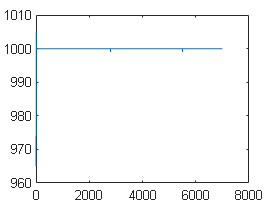
\includegraphics[width=\maxwidth{27.596588058203714em}]{figure_1.png}
\end{center}
\begin{matlabcode}
figure; plot(DLL_filter);
\end{matlabcode}
\begin{center}
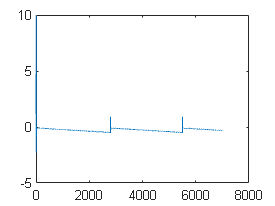
\includegraphics[width=\maxwidth{27.596588058203714em}]{figure_2.png}
\end{center}
\begin{matlabcode}
figure; plot(cd_out);
\end{matlabcode}
\begin{center}
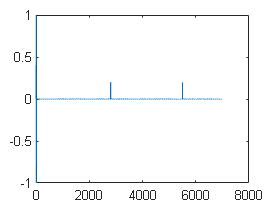
\includegraphics[width=\maxwidth{27.596588058203714em}]{figure_3.png}
\end{center}


\begin{matlabcode}
figure
subplot(2,2,1)
plot(IE)
subplot(2,2,2)
plot(IL)
subplot(2,2,3)
plot(QE)
subplot(2,2,4)
plot(QL)
\end{matlabcode}
\begin{center}
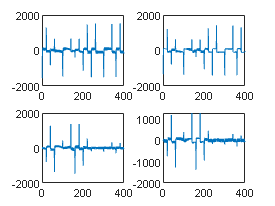
\includegraphics[width=\maxwidth{27.596588058203714em}]{figure_4.png}
\end{center}


\begin{matlabcode}
close all;
\end{matlabcode}


\begin{matlabcode}
figure
subplot(2,2,1)
plot(real(IQ))
subplot(2,2,2)
plot(real(nco_out))
subplot(2,2,3)
plot(imag(IQ))
subplot(2,2,4)
plot(imag(nco_out))
\end{matlabcode}
\begin{center}
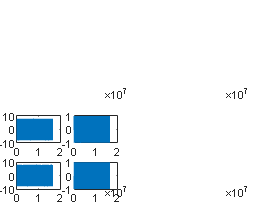
\includegraphics[width=\maxwidth{27.596588058203714em}]{figure_5.png}
\end{center}


\begin{matlabcode}
out_data = zeros(1,length(IQ)+1);

for i = 1:length(IQ)
    out_data(i+1) = out_data(i) + .75*(IQ_data(i) - out_data(i));
end

figure
subplot(2,2,1)
plot(real(IQ.*gc.*nco_out))
subplot(2,2,3)
plot(imag(IQ.*gc.*nco_out))
subplot(2,2,2)
plot(real(out_data(2:end)))
subplot(2,2,4)
plot(imag(out_data(2:end)))
\end{matlabcode}
\begin{center}
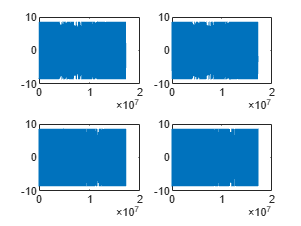
\includegraphics[width=\maxwidth{30.205720020070245em}]{figure_6.png}
\end{center}


\begin{matlabcode}
figure;
subplot(2,1,1)
plot(IP)
subplot(2,1,2)
plot(QP)
\end{matlabcode}
\begin{center}
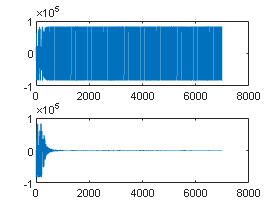
\includegraphics[width=\maxwidth{27.596588058203714em}]{figure_7.png}
\end{center}


\begin{matlabcode}
figure;
subplot(2,1,1)
plot(gc_p)
subplot(2,1,2)
plot(I(end-10230:end))
\end{matlabcode}
\begin{center}
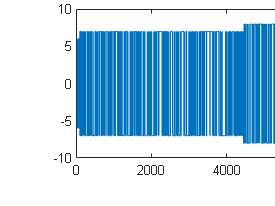
\includegraphics[width=\maxwidth{27.596588058203714em}]{figure_8.png}
\end{center}

\end{document}
